\documentclass[10pt,a4paper]{article}

\usepackage[margin=0.75cm]{geometry}
\usepackage[utf8]{inputenc}

\usepackage{amsmath}
\usepackage{amssymb}
\usepackage[backend=biber]{biblatex}
\usepackage{textcomp}
\usepackage{gensymb}
\usepackage{paracol}
\usepackage{parskip}
\usepackage{tikz}
\usepackage{titlesec}
\usepackage{verbatim}
\usepackage{xcolor}

\titleformat{\section}[block]{\Large\bfseries\filcenter\color{red}}{\thesection}{1em}{}[\hrule]
\titleformat{\subsection}[block]{\bfseries\filcenter\color{red}}{\thesubsection}{1em}{}[\hrule]

\setlength{\columnsep}{25pt}

\tikzset{
    rounded-box/.style = {draw=red, fill=white, thin, rectangle, rounded corners, inner sep=5pt, inner ysep=10pt},
    rounded-box-title/.style = {fill=red, text=white, font=\bfseries},
}

\addbibresource{references.bib}

\begin{document}
\title{Algebra}

\section{Relations}

\begin{paracol}{2}

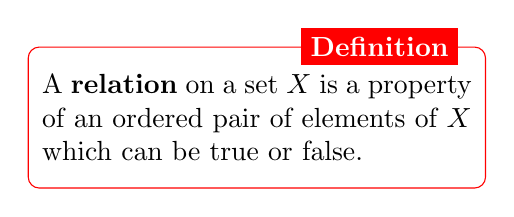
\begin{tikzpicture}
\node [rounded-box] (box){\begin{minipage}{0.45\textwidth}
    A \textbf{relation} on a set $X$ is a property of an ordered pair of elements of $X$ which can be true or false.
\end{minipage}};
\node[rounded-box-title, left=10pt] at (box.north east) {Definition};
\end{tikzpicture}

\textbf{Example}: $<$ is a relation on the set of natural numbers: if $a$ and $b$ are natural numbers then $a < b$ is either true or false.

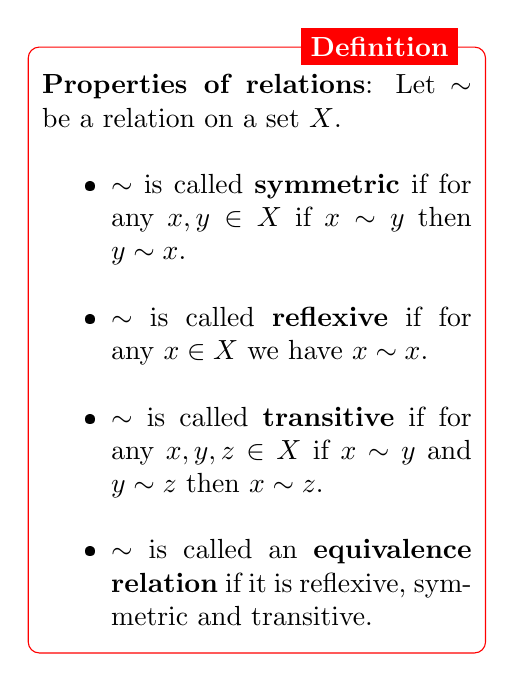
\begin{tikzpicture}
\node [rounded-box] (box){\begin{minipage}{0.45\textwidth}
    \textbf{Properties of relations}: Let $\sim$ be a relation on a set $X$. \\

    \begin{itemize}
        \item $\sim$ is called \textbf{symmetric} if for any $x, y \in X$ if $x \sim y$ then $y \sim x$. \\

        \item $\sim$ is called \textbf{reflexive} if for any $x \in X$ we have $x \sim x$. \\

        \item $\sim$ is called \textbf{transitive} if for any $x, y, z \in X$ if $x \sim y$ and $y \sim z$ then $x \sim z$. \\

        \item $\sim$ is called an \textbf{equivalence relation} if it is reflexive, symmetric and transitive.
    \end{itemize}
\end{minipage}};
\node[rounded-box-title, left=10pt] at (box.north east) {Definition};
\end{tikzpicture}

\switchcolumn

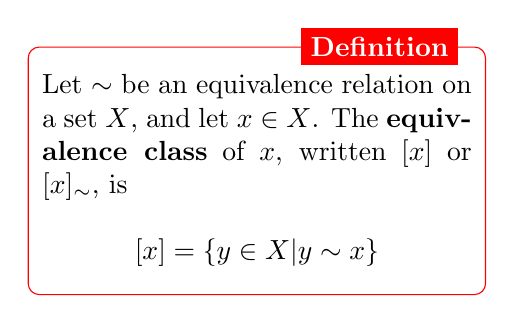
\begin{tikzpicture}
\node [rounded-box] (box){\begin{minipage}{0.45\textwidth}
    Let $\sim$ be an equivalence relation on a set $X$, and let $x \in X$. The \textbf{equivalence class} of $x$, written $[x]$ or $[x]_\sim$, is

    $$[x] = \{ y \in X | y \sim x \}$$
\end{minipage}};
\node[rounded-box-title, left=10pt] at (box.north east) {Definition};
\end{tikzpicture}

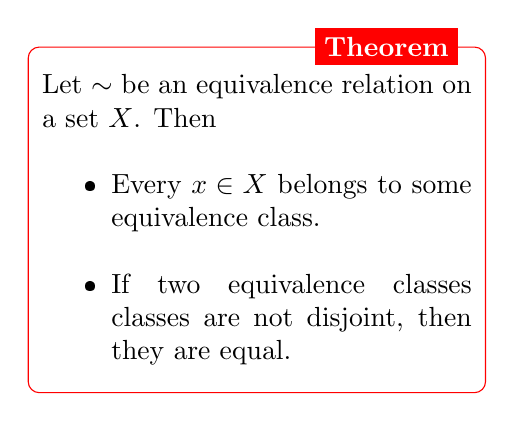
\begin{tikzpicture}
\node [rounded-box] (box){\begin{minipage}{0.45\textwidth}
    Let $\sim$ be an equivalence relation on a set $X$. Then \\

    \begin{itemize}
        \item Every $x \in X$ belongs to some equivalence class. \\

        \item If two equivalence classes classes are not disjoint, then they are equal.
    \end{itemize}
\end{minipage}};
\node[rounded-box-title, left=10pt] at (box.north east) {Theorem};
\end{tikzpicture}

\end{paracol}

\section{Functions}

\begin{paracol}{2}

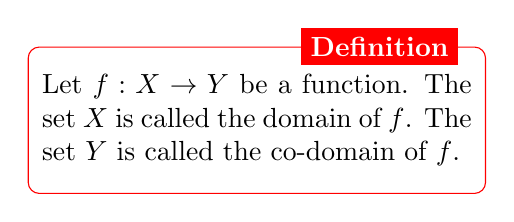
\begin{tikzpicture}
\node [rounded-box] (box){\begin{minipage}{0.45\textwidth}
    Let $f: X \rightarrow Y$ be a function. The set $X$ is called the domain of $f$. The set $Y$ is called the co-domain of $f$.
\end{minipage}};
\node[rounded-box-title, left=10pt] at (box.north east) {Definition};
\end{tikzpicture}

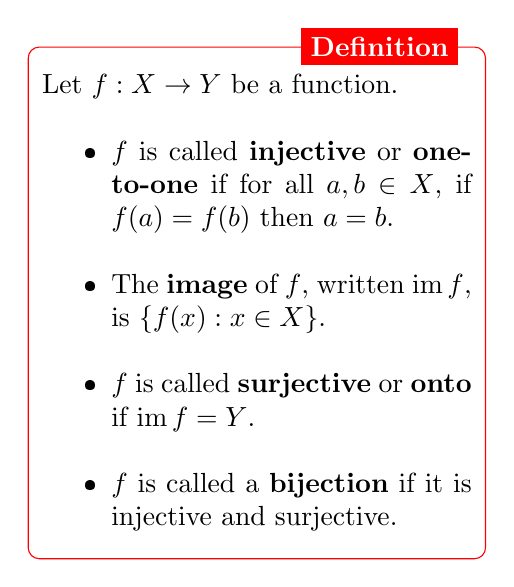
\begin{tikzpicture}
\node [rounded-box] (box){\begin{minipage}{0.45\textwidth}
    Let $f: X \rightarrow Y$ be a function. \\

    \begin{itemize}
        \item $f$ is called \textbf{injective} or \textbf{one-to-one} if for all $a, b \in X$, if $f(a) = f(b)$ then $a = b$. \\

        \item The \textbf{image} of $f$, written $\text{im} \, f$, is $\{ f(x) : x \in X \}$. \\

        \item $f$ is called \textbf{surjective} or \textbf{onto} if $\text{im} \, f = Y$. \\

        \item $f$ is called a \textbf{bijection} if it is injective and surjective.
    \end{itemize}
\end{minipage}};
\node[rounded-box-title, left=10pt] at (box.north east) {Definition};
\end{tikzpicture}

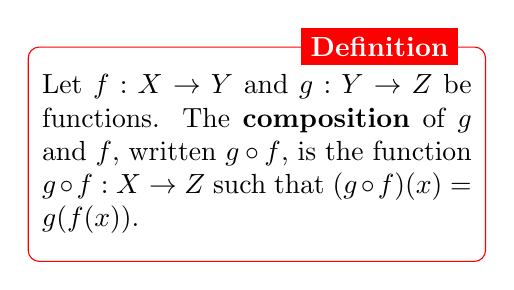
\begin{tikzpicture}
\node [rounded-box] (box){\begin{minipage}{0.45\textwidth}
    Let $f: X \rightarrow Y$ and $g: Y \rightarrow Z$ be functions. The \textbf{composition} of $g$ and $f$, written $g \circ f$, is the function $g \circ f : X \rightarrow Z$ such that $(g \circ f)(x) = g(f(x))$.
\end{minipage}};
\node[rounded-box-title, left=10pt] at (box.north east) {Definition};
\end{tikzpicture}

NB: Composition only makes sense when the co-domain of $f$ is the same as the domain of $g$.

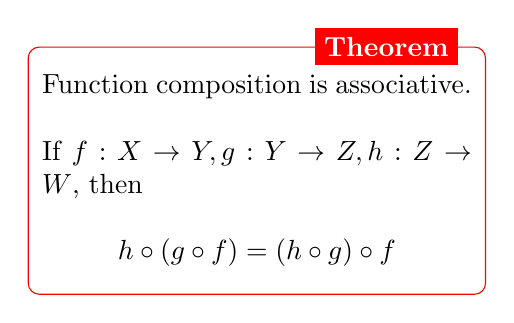
\begin{tikzpicture}
\node [rounded-box] (box){\begin{minipage}{0.45\textwidth}
    Function composition is associative. \\

    If $f: X \rightarrow Y, g: Y \rightarrow Z, h: Z \rightarrow W$, then

    $$h \circ (g \circ f) = (h \circ g) \circ f$$
\end{minipage}};
\node[rounded-box-title, left=10pt] at (box.north east) {Theorem};
\end{tikzpicture}

The reason this is true is because both sides send an input $x \in X$ to the output $h(g(f(x)))$.

\switchcolumn


\begin{tikzpicture}
\node [rounded-box] (box){\begin{minipage}{0.45\textwidth}
    The \textbf{identity function} $\text{id}_X$ does nothing: it is defined by $\text{id}_X(x) = x$ for all $x \in X$.
\end{minipage}};
\node[rounded-box-title, left=10pt] at (box.north east) {Definition};
\end{tikzpicture}

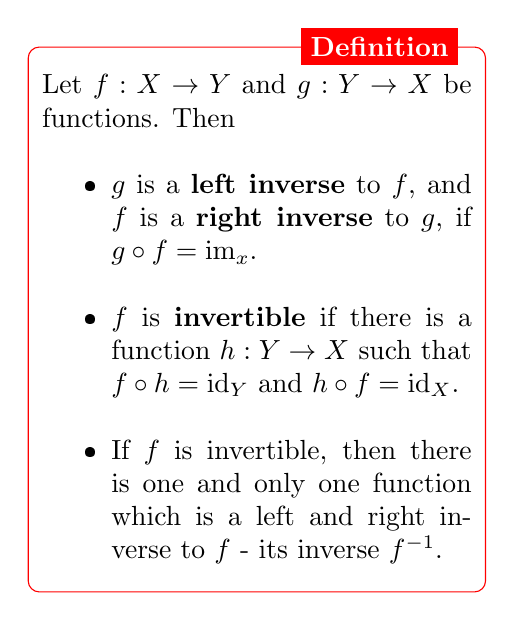
\begin{tikzpicture}
\node [rounded-box] (box){\begin{minipage}{0.45\textwidth}
    Let $f: X \rightarrow Y$ and $g: Y \rightarrow X$ be functions. Then \\

    \begin{itemize}
        \item $g$ is a \textbf{left inverse} to $f$, and $f$ is a \textbf{right inverse} to $g$, if $g \circ f = \text{im}_x$. \\

        \item $f$ is \textbf{invertible} if there is a function $h: Y \rightarrow X$ such that $f \circ h = \text{id}_Y$ and $h \circ f = \text{id}_X$. \\

        \item If $f$ is invertible, then there is one and only one function which is a left and right inverse to $f$ - its inverse $f^{-1}$.
    \end{itemize}
\end{minipage}};
\node[rounded-box-title, left=10pt] at (box.north east) {Definition};
\end{tikzpicture}

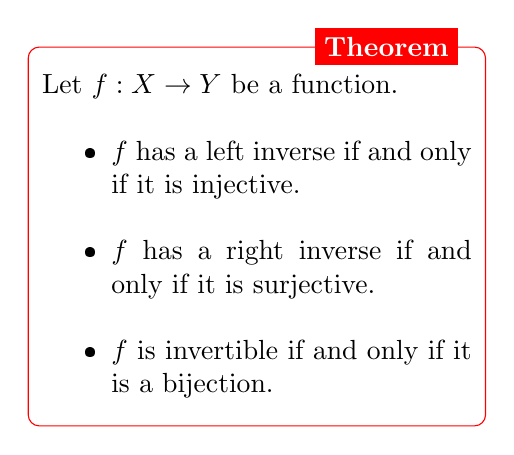
\begin{tikzpicture}
\node [rounded-box] (box){\begin{minipage}{0.45\textwidth}
    Let $f: X \rightarrow Y$ be a function. \\

    \begin{itemize}
        \item $f$ has a left inverse if and only if it is injective. \\

        \item $f$ has a right inverse if and only if it is surjective. \\

        \item $f$ is invertible if and only if it is a bijection.
    \end{itemize}
\end{minipage}};
\node[rounded-box-title, left=10pt] at (box.north east) {Theorem};
\end{tikzpicture}

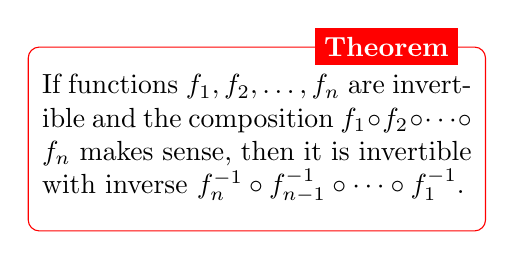
\begin{tikzpicture}
\node [rounded-box] (box){\begin{minipage}{0.45\textwidth}
    If functions $f_1, f_2, \dots, f_n$ are invertible and the composition $f_1 \circ f_2 \circ \dots \circ f_n$ makes sense, then it is invertible with inverse $f_n^{-1} \circ f_{n-1}^{-1} \circ \dots \circ f_1^{-1}$.
\end{minipage}};
\node[rounded-box-title, left=10pt] at (box.north east) {Theorem};
\end{tikzpicture}

\end{paracol}
 \newpage
\section{Permutations}

\begin{paracol}{2}

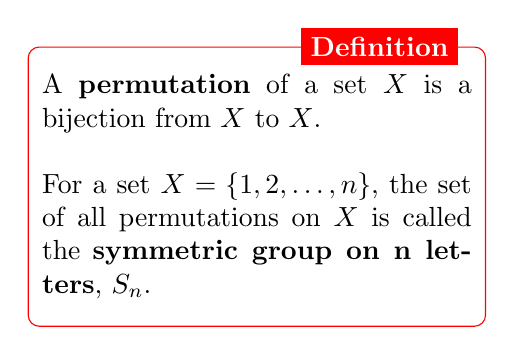
\begin{tikzpicture}
\node [rounded-box] (box){\begin{minipage}{0.45\textwidth}
    A \textbf{permutation} of a set $X$ is a bijection from $X$ to $X$. \\

    For a set $X = \{1, 2, \dots, n\}$, the set of all permutations on $X$ is called the \textbf{symmetric group on n letters}, $S_n$.
\end{minipage}};
\node[rounded-box-title, left=10pt] at (box.north east) {Definition};
\end{tikzpicture}

\switchcolumn

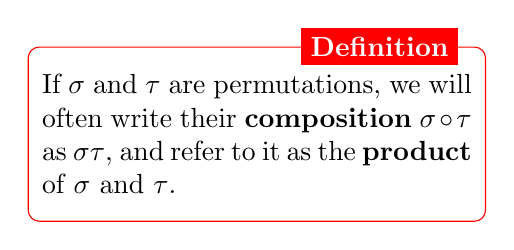
\begin{tikzpicture}
\node [rounded-box] (box){\begin{minipage}{0.45\textwidth}
    If $\sigma$ and $\tau$ are permutations, we will often write their \textbf{composition} $\sigma \circ \tau$ as $\sigma \tau$, and refer to it as the \textbf{product} of $\sigma$ and $\tau$.
\end{minipage}};
\node[rounded-box-title, left=10pt] at (box.north east) {Definition};
\end{tikzpicture}

\end{paracol}

\subsection{Two-row notation}

\begin{paracol}{2}

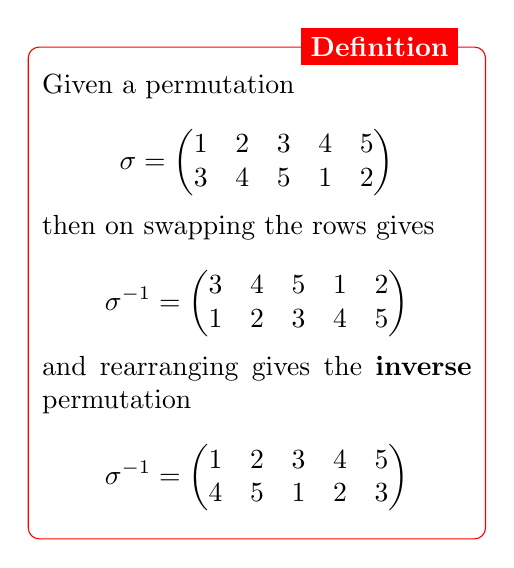
\begin{tikzpicture}
\node [rounded-box] (box){\begin{minipage}{0.45\textwidth}
    Given a permutation

    $$
    \sigma = \begin{pmatrix}
        1 & 2 & 3 & 4 & 5 \\
        3 & 4 & 5 & 1 & 2
    \end{pmatrix}
    $$

    then on swapping the rows gives

    $$
    \sigma^{-1} = \begin{pmatrix}
        3 & 4 & 5 & 1 & 2 \\
        1 & 2 & 3 & 4 & 5
    \end{pmatrix}
    $$

    and rearranging gives the \textbf{inverse} permutation

    $$
    \sigma^{-1} = \begin{pmatrix}
        1 & 2 & 3 & 4 & 5 \\
        4 & 5 & 1 & 2 & 3
    \end{pmatrix}
    $$
\end{minipage}};
\node[rounded-box-title, left=10pt] at (box.north east) {Definition};
\end{tikzpicture}

\switchcolumn

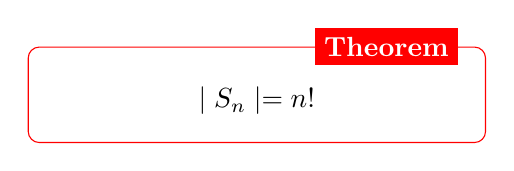
\begin{tikzpicture}
\node [rounded-box] (box){\begin{minipage}{0.45\textwidth}
    $$\mid S_n \mid = n!$$
\end{minipage}};
\node[rounded-box-title, left=10pt] at (box.north east) {Theorem};
\end{tikzpicture}

\textbf{Proof}: Induction on $n$.

When $n = 1$ there is a unique bijection $\{1\} \rightarrow \{1\}$, namely the identity map, so $\mid S_1 \mid = 1 = 1!$ as required.

The number of elements of $S_n$ is the number of different ways to order the elements $1, 2, \dots, n$. An ordering of $1, 2, \dots, n$ is the same thing as an ordering of $1, 2, \dots, n-1$ with $n$ inserted into one of $n$ positions, so the number of possible orderings is $n$ times the number of orderings of $1, \dots, n-1$, which is $(n-1)!$ by the inductive hypothesis.

So $\mid S_n \mid = x \times (n-1)! = n!$.

\end{paracol}

\subsection{Cycles}

\begin{paracol}{2}

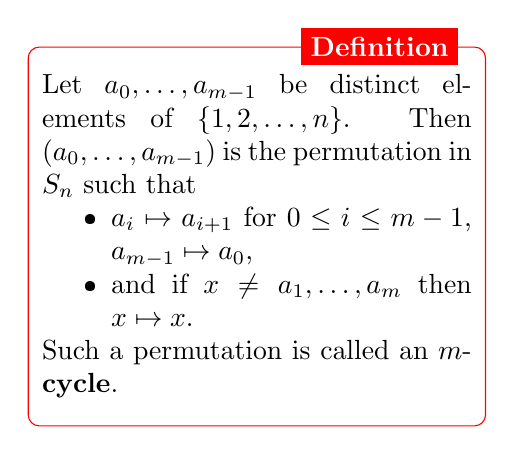
\begin{tikzpicture}
\node [rounded-box] (box){\begin{minipage}{0.45\textwidth}
    Let $a_0, \dots, a_{m-1}$ be distinct elements of $\{1, 2, \dots, n\}$. Then $(a_0, \dots, a_{m-1})$ is the permutation in $S_n$ such that

    \begin{itemize}
        \item $a_i \mapsto a_{i+1}$ for $0 \leq i \leq m-1$, $a_{m-1} \mapsto a_0$,
        \item and if $x \neq a_1, \dots, a_m$ then $x \mapsto x$.
    \end{itemize}

    Such a permutation is called an $m$-\textbf{cycle}.
\end{minipage}};
\node[rounded-box-title, left=10pt] at (box.north east) {Definition};
\end{tikzpicture}

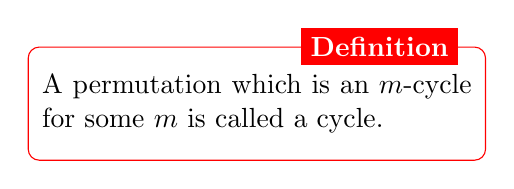
\begin{tikzpicture}
\node [rounded-box] (box){\begin{minipage}{0.45\textwidth}
    A permutation which is an $m$-cycle for some $m$ is called a cycle.
\end{minipage}};
\node[rounded-box-title, left=10pt] at (box.north east) {Definition};
\end{tikzpicture}

\textbf{Counter-example}: Not every permutation is a cycle, e.g. $\begin{pmatrix}
    1 & 2 & 3 & 4 \\
    2 & 1 & 4 & 3
\end{pmatrix}$.

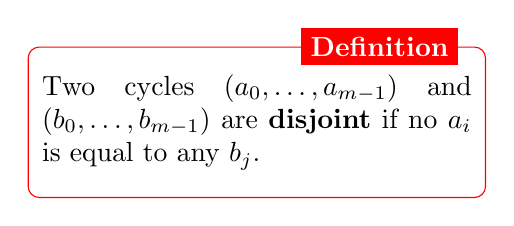
\begin{tikzpicture}
\node [rounded-box] (box){\begin{minipage}{0.45\textwidth}
    Two cycles $(a_0, \dots, a_{m-1})$ and $(b_0, \dots, b_{m-1})$ are \textbf{disjoint} if no $a_i$ is equal to any $b_j$.
\end{minipage}};
\node[rounded-box-title, left=10pt] at (box.north east) {Definition};
\end{tikzpicture}

Any permutation can be written as a product of disjoint cycles, e.g. the permutation above is equal to $(1, 2)(3, 4)$.

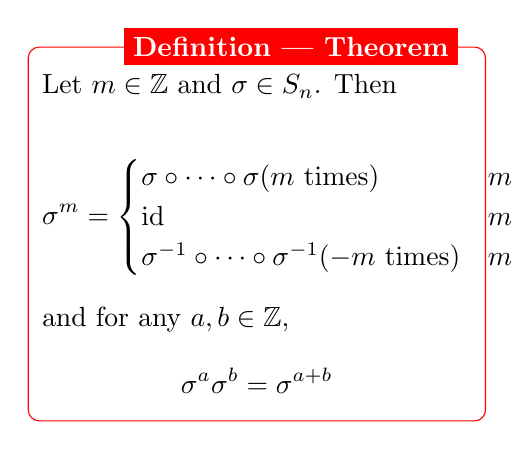
\begin{tikzpicture}
\node [rounded-box] (box){\begin{minipage}{0.45\textwidth}
    Let $m \in \mathbb{Z}$ and $\sigma \in S_n$. Then

    \begin{equation*}
        \sigma^m = \begin{cases}
            \sigma \circ \dots \circ \sigma (m \text{ times}) & m > 0 \\
            \text{id} & m = 0 \\
            \sigma^{-1} \circ \dots \circ \sigma^{-1} (-m \text{ times}) & m < 0 \\
        \end{cases}
    \end{equation*}

    and for any $a, b \in \mathbb{Z}$,

    $$\sigma^a \sigma^b = \sigma^{a+b}$$
\end{minipage}};
\node[rounded-box-title, left=10pt] at (box.north east) {Definition | Theorem};
\end{tikzpicture}

\switchcolumn

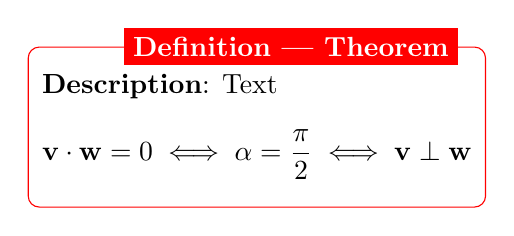
\begin{tikzpicture}
\node [rounded-box] (box){\begin{minipage}{0.45\textwidth}
    \textbf{Description}: Text
    $$\mathbf{v} \cdot \mathbf{w} = 0 \iff \alpha = \frac{\pi}{2} \iff \mathbf{v} \perp \mathbf{w}$$
\end{minipage}};
\node[rounded-box-title, left=10pt] at (box.north east) {Definition | Theorem};
\end{tikzpicture}

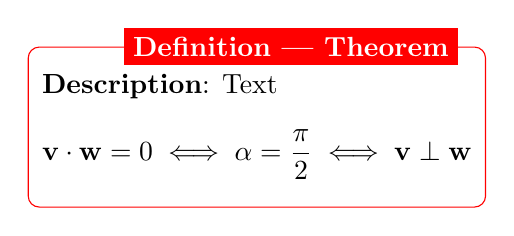
\begin{tikzpicture}
\node [rounded-box] (box){\begin{minipage}{0.45\textwidth}
    \textbf{Description}: Text
    $$\mathbf{v} \cdot \mathbf{w} = 0 \iff \alpha = \frac{\pi}{2} \iff \mathbf{v} \perp \mathbf{w}$$
\end{minipage}};
\node[rounded-box-title, left=10pt] at (box.north east) {Definition | Theorem};
\end{tikzpicture}

\end{paracol}
 \newpage
\section{Groups}

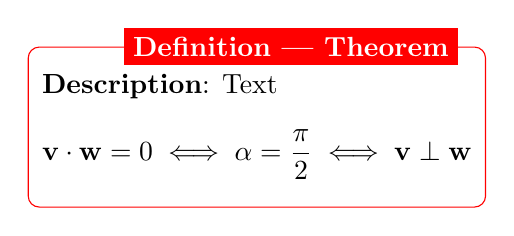
\begin{tikzpicture}
\node [rounded-box] (box){\begin{minipage}{0.45\textwidth}
    \textbf{Description}: Text
    $$\mathbf{v} \cdot \mathbf{w} = 0 \iff \alpha = \frac{\pi}{2} \iff \mathbf{v} \perp \mathbf{w}$$
\end{minipage}};
\node[rounded-box-title, left=10pt] at (box.north east) {Definition | Theorem};
\end{tikzpicture}

\subsection{The Symmetric Group}

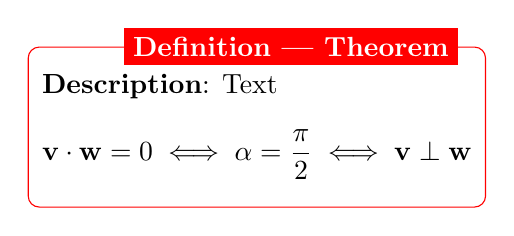
\begin{tikzpicture}
\node [rounded-box] (box){\begin{minipage}{0.45\textwidth}
    \textbf{Description}: Text
    $$\mathbf{v} \cdot \mathbf{w} = 0 \iff \alpha = \frac{\pi}{2} \iff \mathbf{v} \perp \mathbf{w}$$
\end{minipage}};
\node[rounded-box-title, left=10pt] at (box.north east) {Definition | Theorem};
\end{tikzpicture}

\subsection{Subgroups}

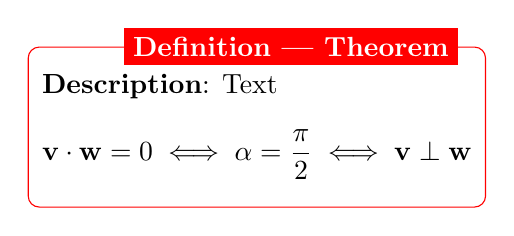
\begin{tikzpicture}
\node [rounded-box] (box){\begin{minipage}{0.45\textwidth}
    \textbf{Description}: Text
    $$\mathbf{v} \cdot \mathbf{w} = 0 \iff \alpha = \frac{\pi}{2} \iff \mathbf{v} \perp \mathbf{w}$$
\end{minipage}};
\node[rounded-box-title, left=10pt] at (box.north east) {Definition | Theorem};
\end{tikzpicture}

\subsection{Cosets and Lagrange's Theorem}

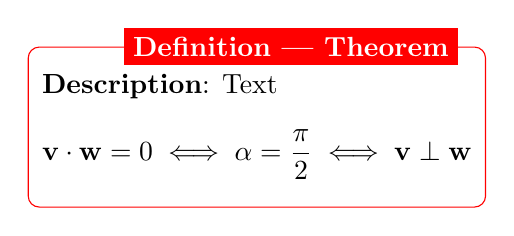
\begin{tikzpicture}
\node [rounded-box] (box){\begin{minipage}{0.45\textwidth}
    \textbf{Description}: Text
    $$\mathbf{v} \cdot \mathbf{w} = 0 \iff \alpha = \frac{\pi}{2} \iff \mathbf{v} \perp \mathbf{w}$$
\end{minipage}};
\node[rounded-box-title, left=10pt] at (box.north east) {Definition | Theorem};
\end{tikzpicture}

\subsection{The Dihedral Groups}

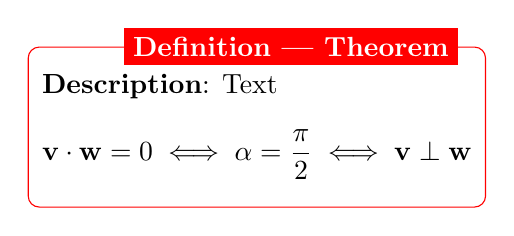
\begin{tikzpicture}
\node [rounded-box] (box){\begin{minipage}{0.45\textwidth}
    \textbf{Description}: Text
    $$\mathbf{v} \cdot \mathbf{w} = 0 \iff \alpha = \frac{\pi}{2} \iff \mathbf{v} \perp \mathbf{w}$$
\end{minipage}};
\node[rounded-box-title, left=10pt] at (box.north east) {Definition | Theorem};
\end{tikzpicture}

\subsection{Homomorphisms and Isomorphisms}

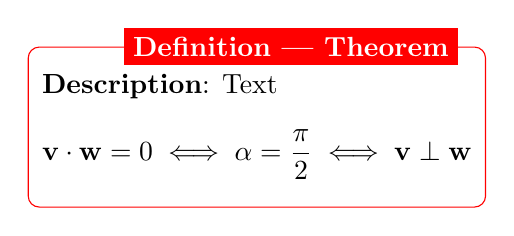
\begin{tikzpicture}
\node [rounded-box] (box){\begin{minipage}{0.45\textwidth}
    \textbf{Description}: Text
    $$\mathbf{v} \cdot \mathbf{w} = 0 \iff \alpha = \frac{\pi}{2} \iff \mathbf{v} \perp \mathbf{w}$$
\end{minipage}};
\node[rounded-box-title, left=10pt] at (box.north east) {Definition | Theorem};
\end{tikzpicture}

 \newpage
\section{Categories}

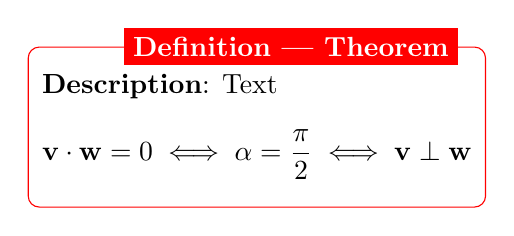
\begin{tikzpicture}
\node [rounded-box] (box){\begin{minipage}{0.45\textwidth}
    \textbf{Description}: Text
    $$\mathbf{v} \cdot \mathbf{w} = 0 \iff \alpha = \frac{\pi}{2} \iff \mathbf{v} \perp \mathbf{w}$$
\end{minipage}};
\node[rounded-box-title, left=10pt] at (box.north east) {Definition | Theorem};
\end{tikzpicture}
 \newpage

\nocite{*}
\printbibliography

\end{document}
